\subsection{Finite state transducers}

A {\em finite state transducer} (FST) is a finite state machine with input and output tapes. 
FSTs differ from {\em finite state automata} (FSA) in that
they have an output tape while FSAs have accept states instead.

Formally, an FST is a tuple $M = (S,S_{0},\sigma,\varGamma,\delta)$ where $S$ is the set of states,
$S_{0} \subset S$ is the set of initial states, 
$\sigma$ is the input alphabet, 
$\varGamma$ is the output alphabet, 
and $\delta \subseteq S \times (\sigma \times \{\epsilon\}) \times (\varGamma \times \{\epsilon\}) \times S$ is the transition relation.

FSTs have been used extensively in text mining applications where the input is the text and the output is the
delimiters of a chunk of text with an associated class~\cite{beesley2001finite}. 
FSTs are attractive in NLP tasks due to their efficiency and ease of use.

\subsection{Classes, labels, and tag types}

A {\em class} is a semantic decision that the NLP of CL task tries to make. 
Parts of text that belong to the desired class are all assigned the same class {\em label}. 
For example, {\em temporal unit} is a label of a class that encompasses explicit temporal 
information in the sentence related to time such as 
\RL{dqyqT} (minute) and \RL{sA`T} (hour). 

The user may wish to define a simple class as an abstract category that contains a 
set of morphemes. 
For more sophisticated classes, the user can use the visual interface in \framework to 
define the class through Boolean formulae with morphology-based atomic terms. 
The annotation of text with the labels of the classes can later be used in 
CL and NLP tasks for learning, testing, and validation.

\subsection{Analysis}

In addition to automatic and manual tagging, \framework 
allows comparing tag sets and tag types applied to the
same input text. 
The \framework comparator takes as input two tag sets $R_1$ and $R_2$ and 
two tag type sets ${\cal T}_1$ and ${\cal T}_2$. 
It produces a difference view for the tag types and 
a difference view for the tag sets. 
The tag type difference view shows the common tag types ${\cal T}_1 \cap {\cal T}_2$,
the tag types in ${\cal T}_1$ and not in ${\cal T}_2$, 
and the tag types in ${\cal T}_2$ and not in ${\cal T}_1$.

Similarly, the tag set difference view shows $R_1\cap R_2$, $R_1/R_2$ and $R_2/R_1$. 
The tag set difference view, as shown in Figure~\ref{f:diff} also shows the precision, 
recall and F-measure between the two sets. 
The metrics can be computed based on several predicates. 
The ``Intersection'' predicate returns true if a tag from $R_1$ intersects in text $T$ 
with a tag in $R_2$. 
The ``Exact'' predicate returns true if a tag from $R_1$ exactly matches a tag
in $R_2$. 
The ``A includes B'' predicate returns true if a tag from $R_1$ contains a tag from $R_2$. 
Finally, the ``B includes A'' predicate returns true if a tag from $R_2$ contains 
a tag from $R_1$. 

In the difference view panes, the user can select a difference tag and accept it, or reject
it to build a corrected corpora.

\begin{figure*}[tb!]
  \centering
  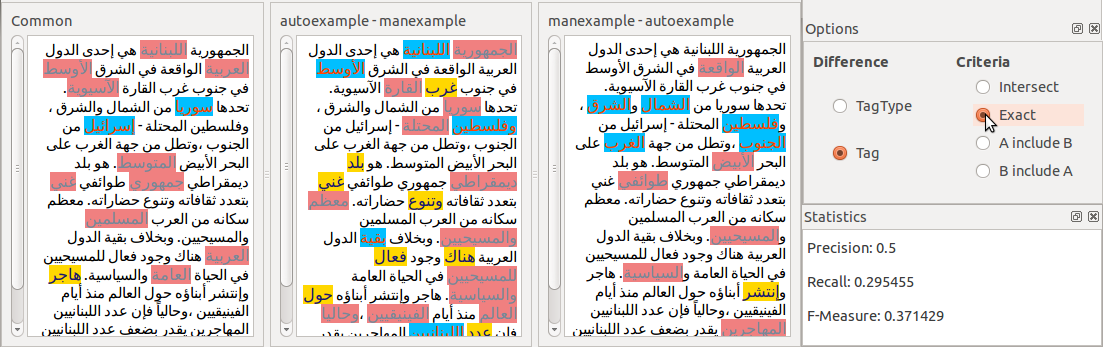
\includegraphics[width=\textwidth]{figures/diff}
  \caption{\framework comparison and accuracy results view.}
  \label{f:diff}
\end{figure*}
